
\newpage 

\section{Stack Data Structures}
\label{sec:stacks_heaps}

\noindent
Let's talk about our first data structure, the stack:
\begin{Def}[Stack]

    A \textbf{stack data structure} is a collection of elements that follows a \textbf{Last In, First Out} (LIFO) principle. I.e., in a 
    stack of plates, the last added plate is the first one to be removed, not the middle or bottom/first plate.
    Each \textit{plate} in the stack is called a \textbf{stack frame}.\\

    \noindent
    A \textbf{call stack} is a stack which keeps track of function calls in a program as well as any local variables within such functions.
    
    \underline{This is why we say a variable is in \textbf{scope}}, as when a function is taken off the stack, or a new stack frame 
    is placed on top, the variables in the previous or discarded stack frame are \textbf{no longer accessible}.
\end{Def}

\vspace{-1.5em}

\begin{figure}[ht!]
    \centering
    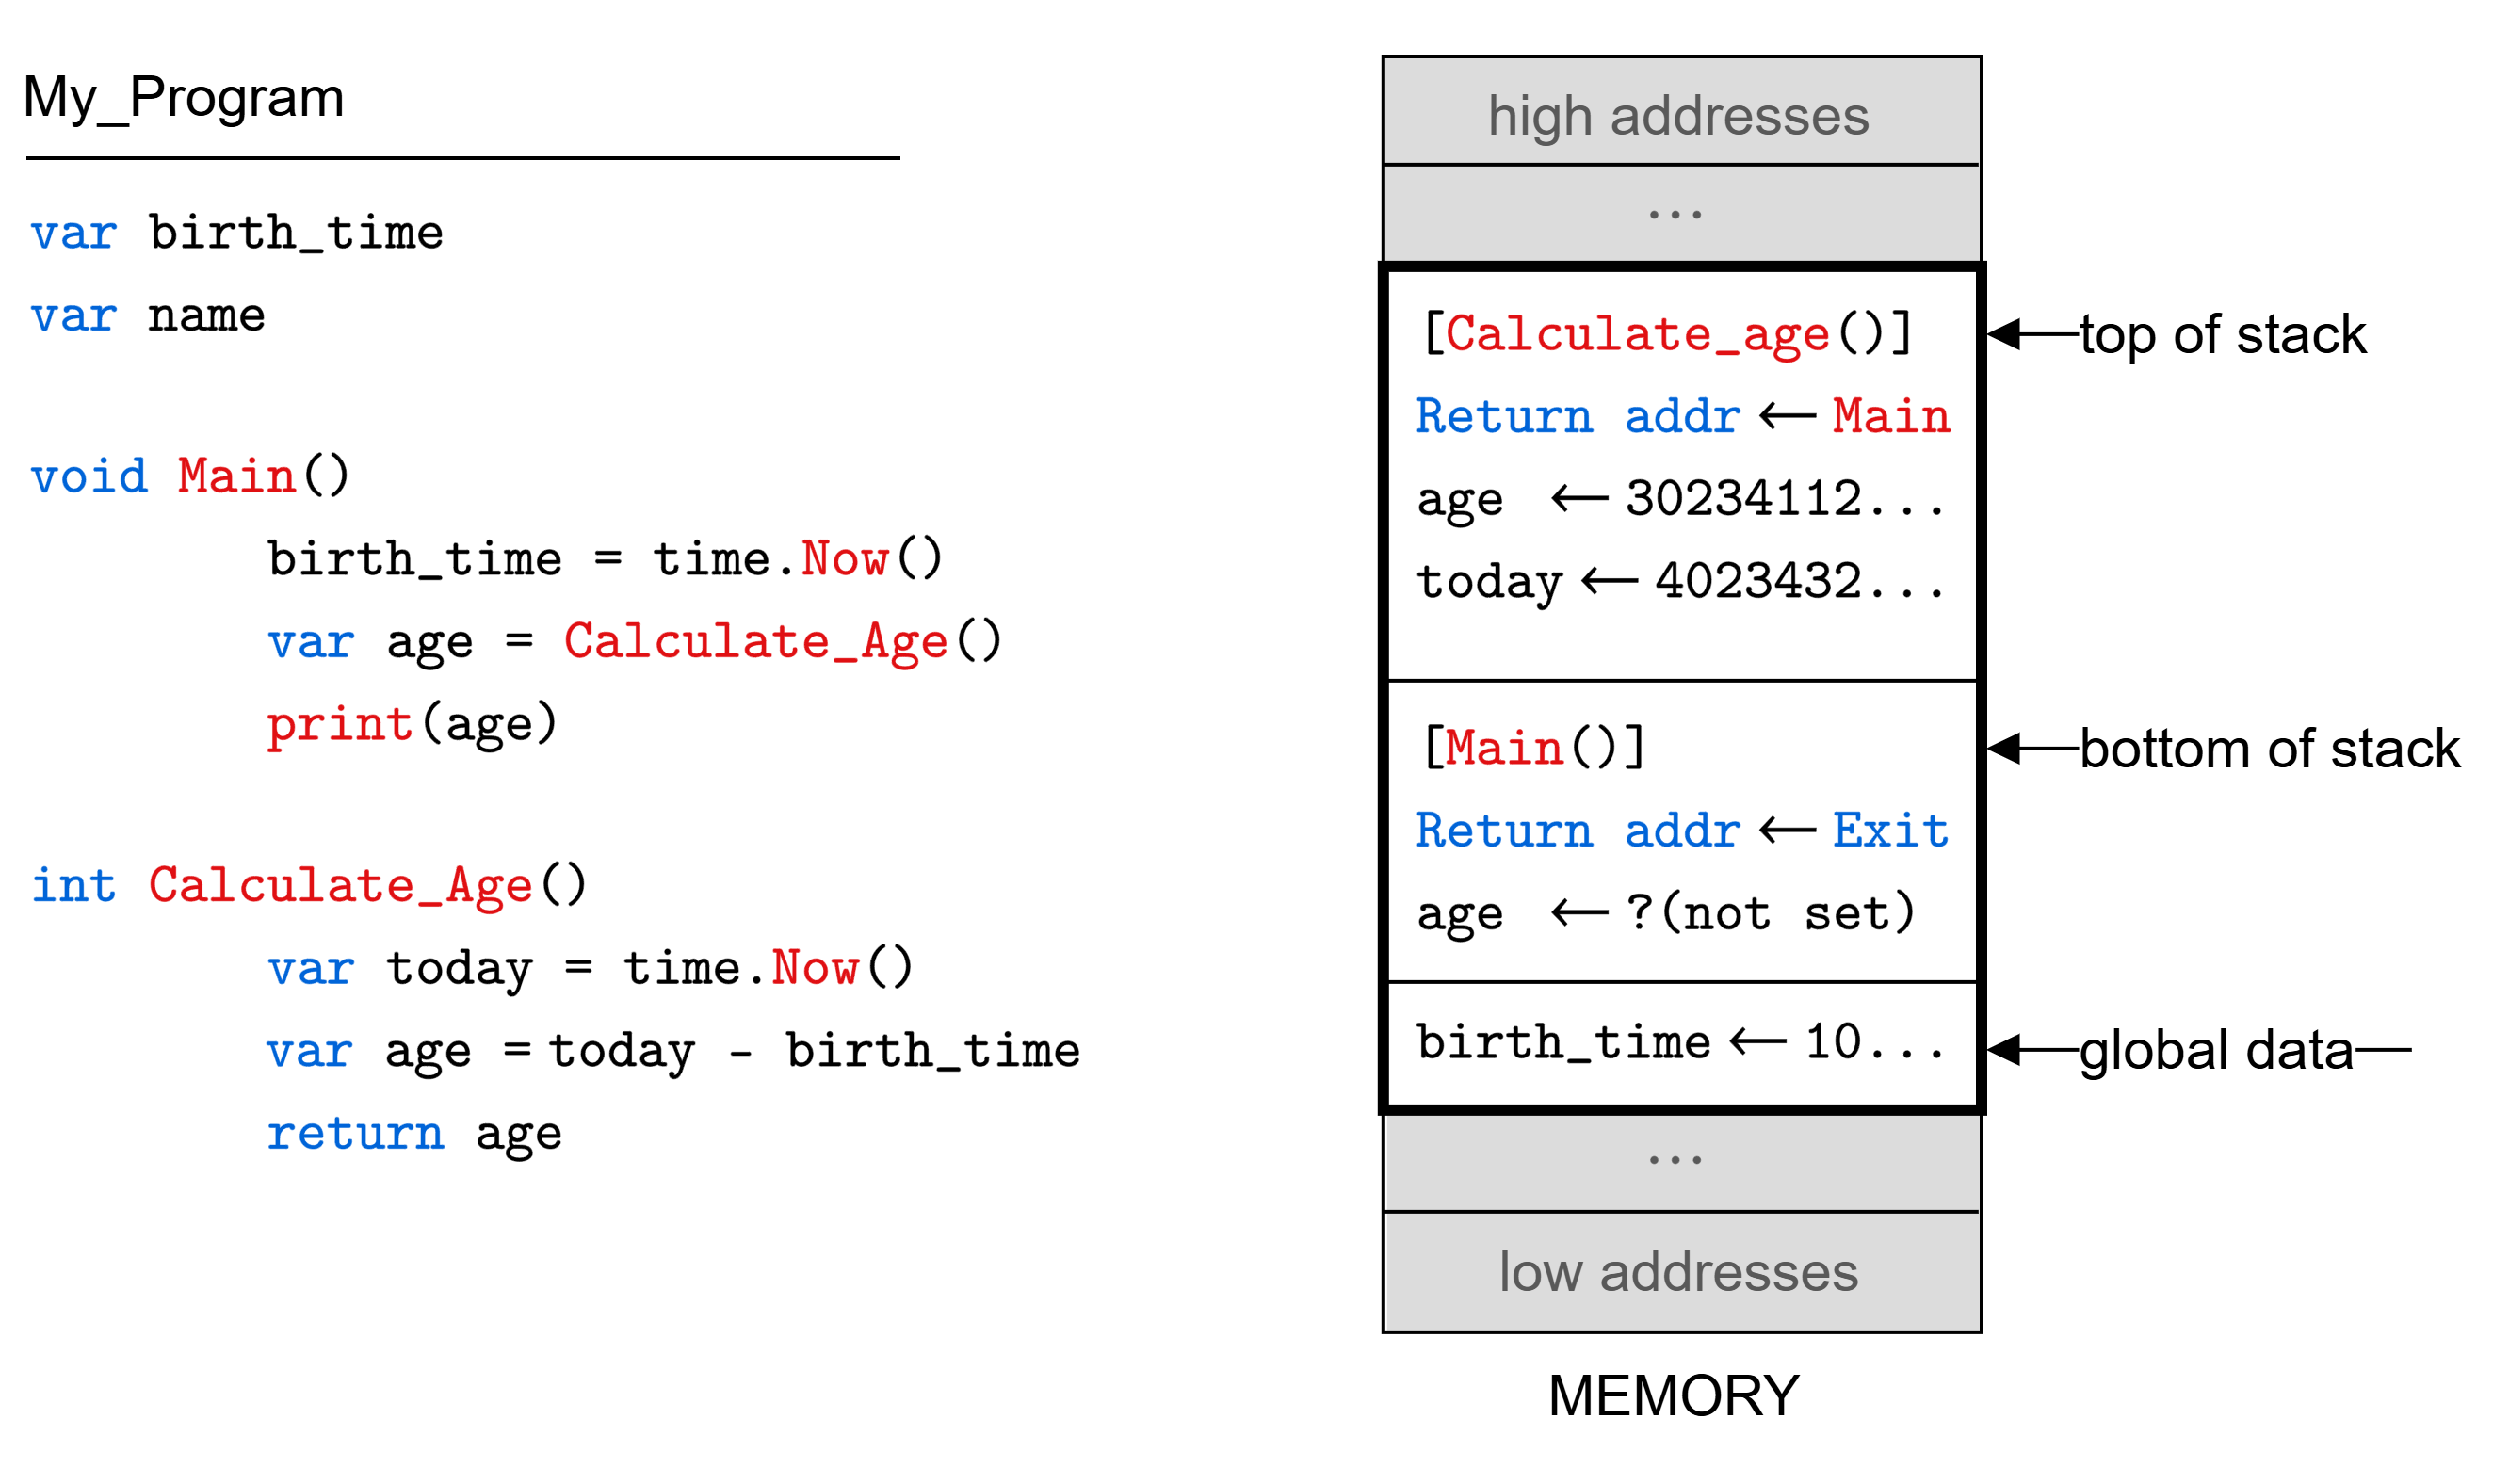
\includegraphics[width=0.8\textwidth]{./Sections/stacks_heaps/call_stack.png}
    \caption{Here is a simplified look at how memory manages the stack. On the left is our program written 
    in some abstract language, and on the right is the call stack in memory (simplified). 
    The program has a global `birth\_time' variable, which is initialized in the \texttt{Main} function. The \texttt{Main} function
    then calls the \texttt{Calculate\_Age} function which uses the `birth\_time' variable to calculate the `age' via the difference of 
    the current time and the `birth\_time.'
    Looking at the memory, we see at the bottom of our memory contains global variables accessible to any frame. Next, is the bottom of the stack, containing a return address to exit 
    the program, while awaiting the result of the function call for `age'. The top of our stack contains another frame that we will return the value
    a new `age' (not the same as the one before) not accessible from the main function. This new frame also contains a new local variable `today.'
    Once this function returns, \texttt{Main} will have the result of its local variable `age.'. Concretely, the 
    `age' variable in both the \texttt{Main} and \texttt{Calculate\_Age} function are completely separate despite sharing the same \textit{name}.}
    \label{fig:call_stack}
\end{figure}

\newpage 

\noindent
\underline{\textbf{Please Note:} The above figure is a simplified version}; This presentation derivatives from what actually happens
for teaching sake. In the following pages we define the stack frame in more detail.

\begin{Tip}
A lot of demonstrations (including this text) will show the stack growing \textbf{upwards}; This is strictly because it's easier to visualize and does not
accurately portray what a stack really does or looks like. In the following pages we will clear this up, and show how the stack actually grows from top-to-bottom.
Of course, there is always room for deviation if a developer wishes to implement a stack in some other arbitrary way. Nonetheless, the following is what one 
might typically expect in a stack implementation.
\end{Tip}

\begin{Def}[Stack Frame Anatomy]

Under the x86-32 calling convention Two registers keep track our place in the stack:
\begin{itemize}
  \item \textbf{Base Pointer (BP/EBP):} Points to the base (i.e.\ ``bottom'') of the current function's stack frame.
  \item \textbf{Stack Pointer (SP/ESP):} Points to the ``top'' of the current function's stack frame, i.e., the next free byte where a push would land.
\end{itemize}

\noindent
When the program starts, the operating system \emph{reserves} a contiguous region of memory for the stack. By convention, the \emph{bottom} of that region lies at a higher address, 
and the stack ``grows downward'' toward lower addresses as data is pushed. If the stack pointer ever moves past the reserved limit---a \textbf{stack overflow} occurs.
\\

\noindent
A single \textbf{stack frame} itself is a contiguous block of memory in which the function stores:
\begin{itemize}
  \item \textbf{Parameters:} The arguments passed in by the caller,  
  \item \textbf{Return Address:} The address of the next instruction to execute after the function returns,
  \item \textbf{Old Base Pointer:} The caller's `EBP', saved so that on return we can restore the previous frame,
  \item \textbf{Local Variables:} Space for any locals or temporaries that the function needs.  
\end{itemize}

\noindent
This is why variables in previous or new functions calls become ``\textbf{out of scope}'' (no longer accessible), as they belong to some other stack frame; 
When it comes to \textbf{Global Variables}, they live in a separate region of memory, defined by the \textbf{data segment} (\ref{def:machine_code}).

Moreover, a call to a new function invokes the \underline{\textbf{call} instruction}, this automatically pushes the return address to the current frame onto the stack.
Additionally, the CPU reserves the \textbf{EAX} register for the return value (number or address) of a function. 
When the function returns, it can place its result in `EAX', and the caller can retrieve it from there. During constant use 
the `EAX' \underline{register may contain \textbf{garbage}} data from previous use, unless explicitly set to zero or some other value.
\end{Def}

\newpage 

\begin{table}[h]
\centering
\resizebox{\textwidth}{!}{
\begin{tabular}{|c|c|l|}
\hline
\multicolumn{3}{|c|}{\textbf{High Addresses}} \\ \hline
\textbf{Contents}       & \textbf{Offset} & \textbf{Notes} \\
\hline
\emph{(Parameters 3, 4, \(\dots\))} & \(\mathit{EBP} + 16\), \(+20\), \(\dots\) & Third-and-onward arguments, if any. \\ 
Parameter 2            & \(\mathit{EBP} + 12\) & Second argument passed on stack. \\
Parameter 1            & \(\mathit{EBP} + 8\)  & First argument passed on stack. \\
Return Address         & \(\mathit{EBP} + 4\)  & Auto-pushed by the \texttt{call} instruction.\\
Old EBP (Saved BP)     & \(\mathit{EBP} + 0\)  & The caller's base pointer \\
\hline
\multicolumn{3}{|c|}{\textbf{Current Frame (locals/temporaries)}} \\ \hline
Local Variable 1        & \(\mathit{EBP} - 4\)  & First 4-byte local (or smallest slot). \\
Local Variable 2        & \(\mathit{EBP} - 8\)  & Next 4-byte local or part of a larger object. \\
\(\dots\)                      & \( \vdots \)         &(additional locals at \(\mathit{EBP} - 12,\ -16,\ \dots\)) \\
\hline
\multicolumn{3}{|c|}{\textbf{Low Addresses}} \\ \hline
\end{tabular}
}
\caption{Typical x86-32 Stack-Frame Layout, where offsets are typically a multiple of 4 bytes.}
\end{table}

\begin{figure}[!ht]
    \centering
    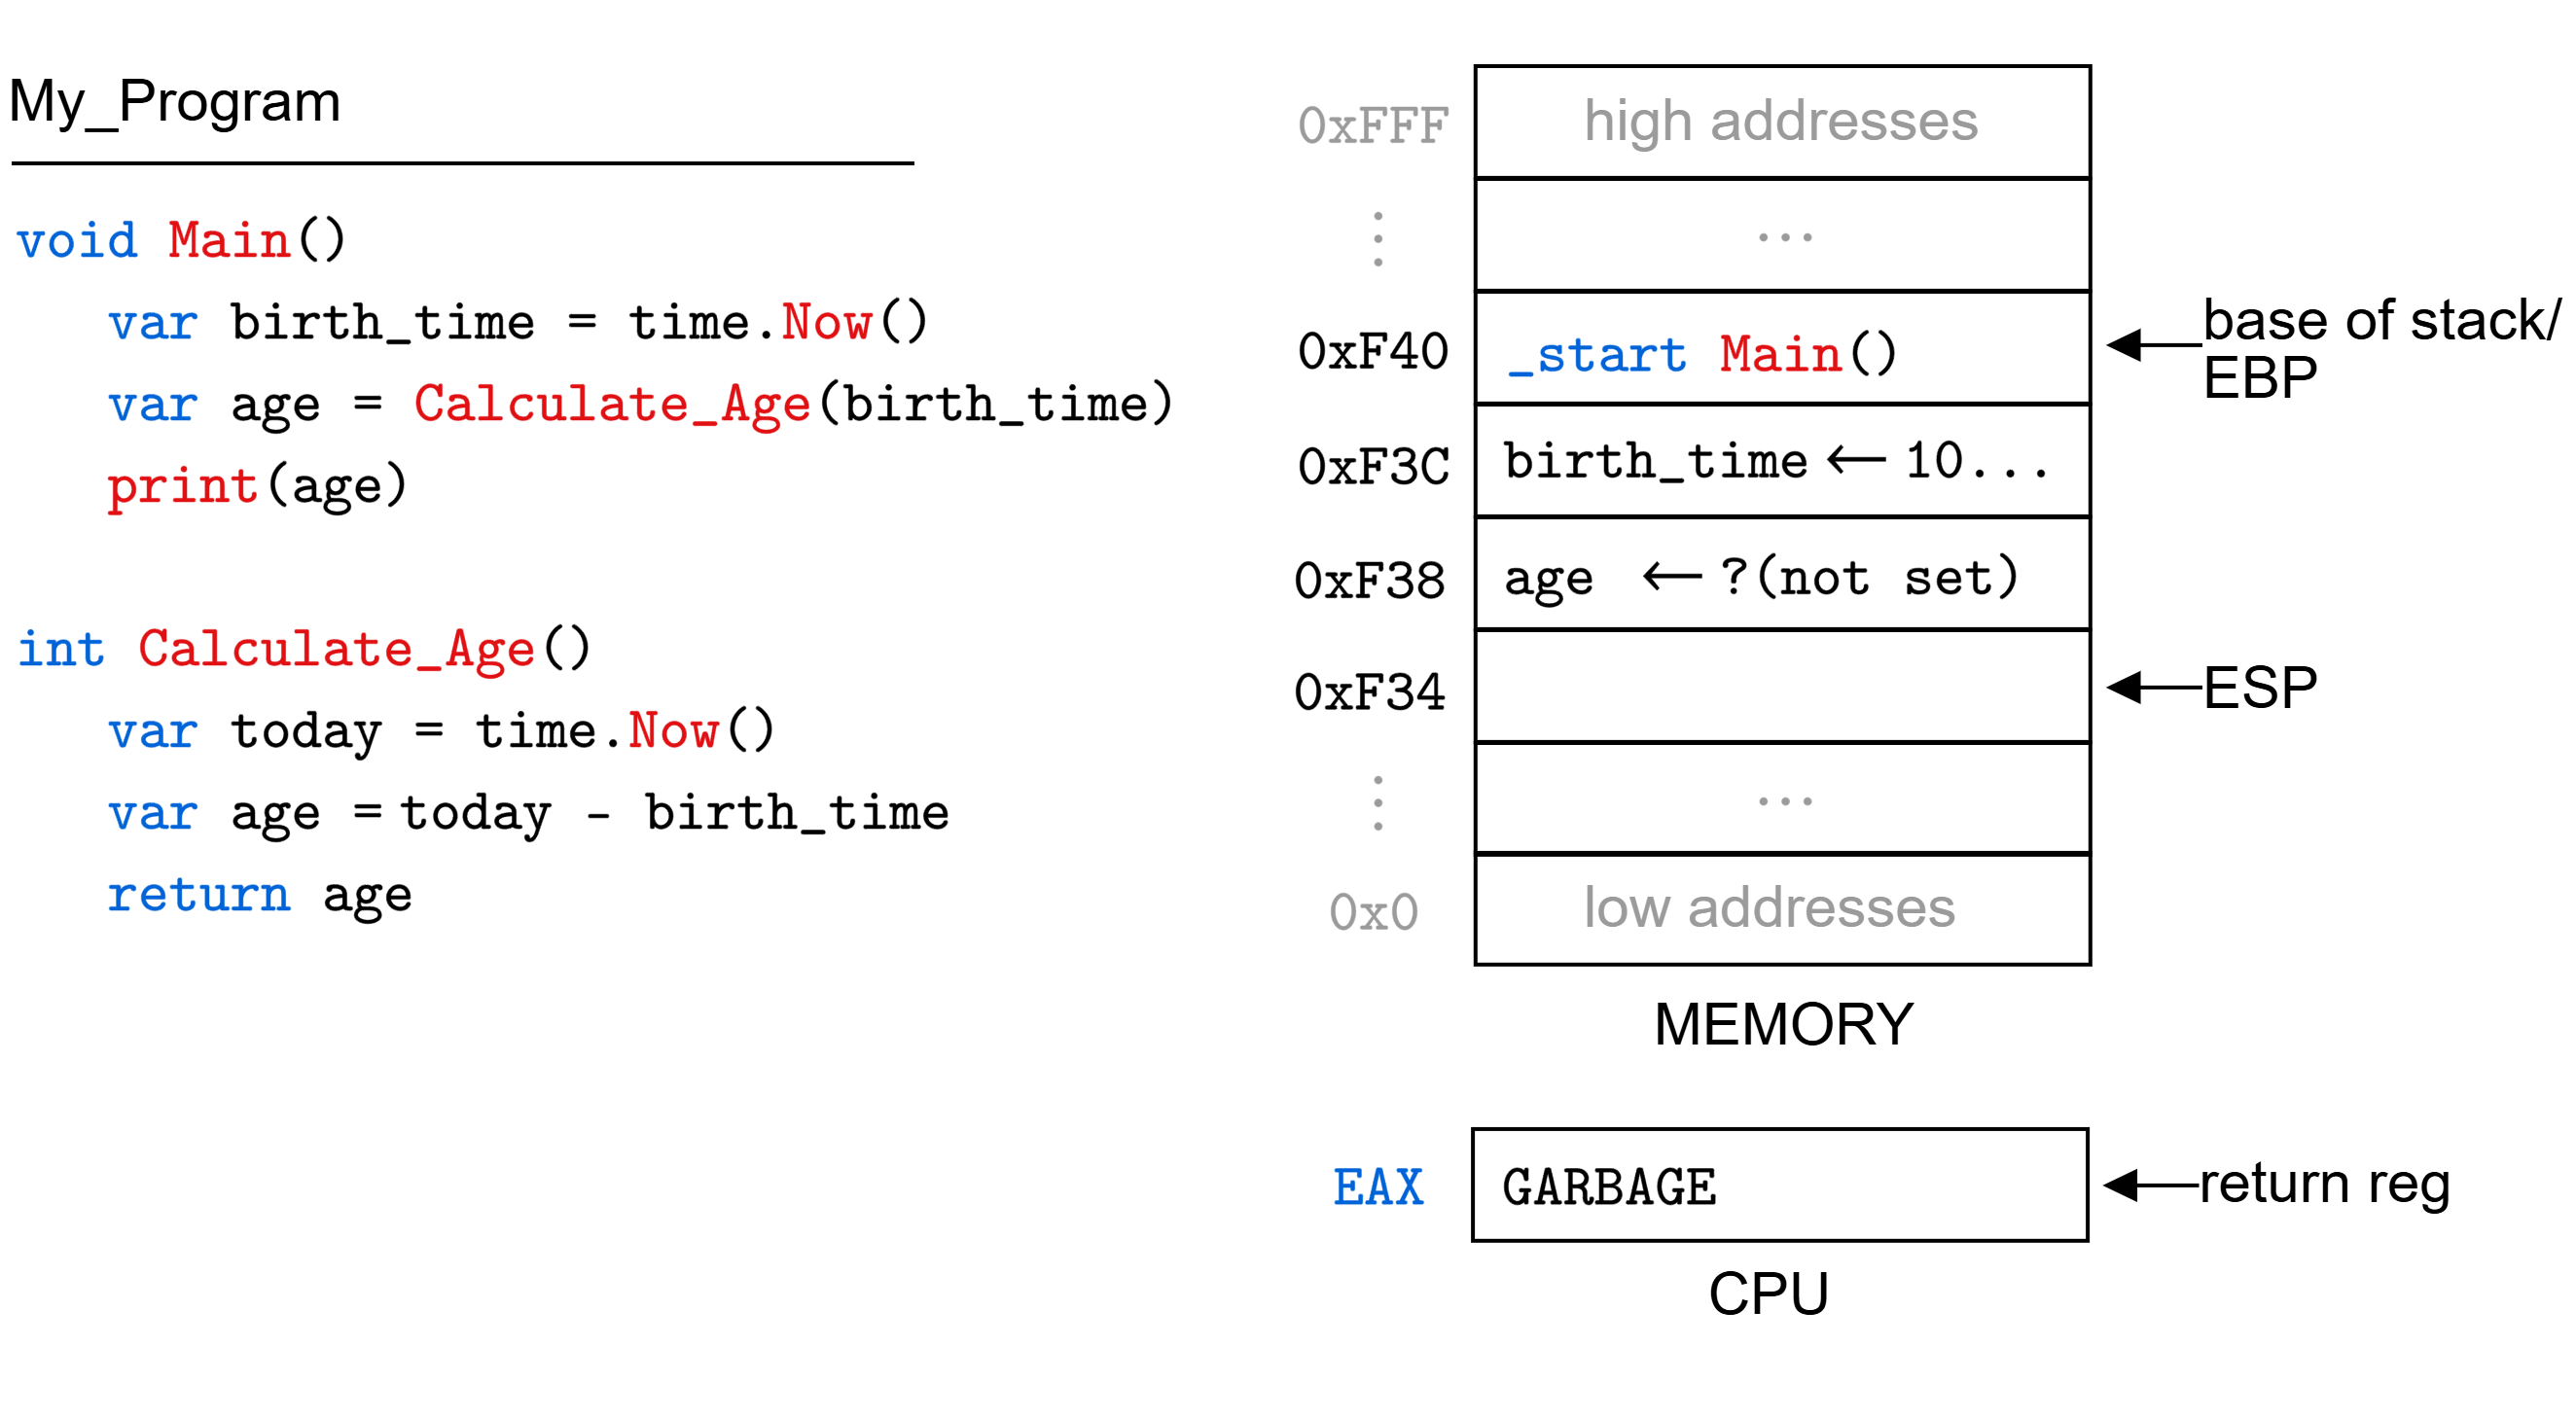
\includegraphics[width=\textwidth]{./Sections/stacks_heaps/call_stack_precise.png}
    \caption{Revisiting Figure (\ref{fig:call_stack}) with slight alterations to the code: This is a snapshot of the code executing right before \texttt{CalculateAge(birth\_time)} is called. For simplicity sake,
    let's say the stack begins at address \texttt{0xF40} (Hexadecimal), growing downwards. Here the base of the stack and the EBP are one and the same.
    We include the CPU's EAX (return register), which contains garbage. Address \texttt{0xF38} is currently just reserved space for `age'.}

\label{fig:call_stack_precise}
\end{figure}

\newpage 

\begin{figure}[!ht]
    \centering
    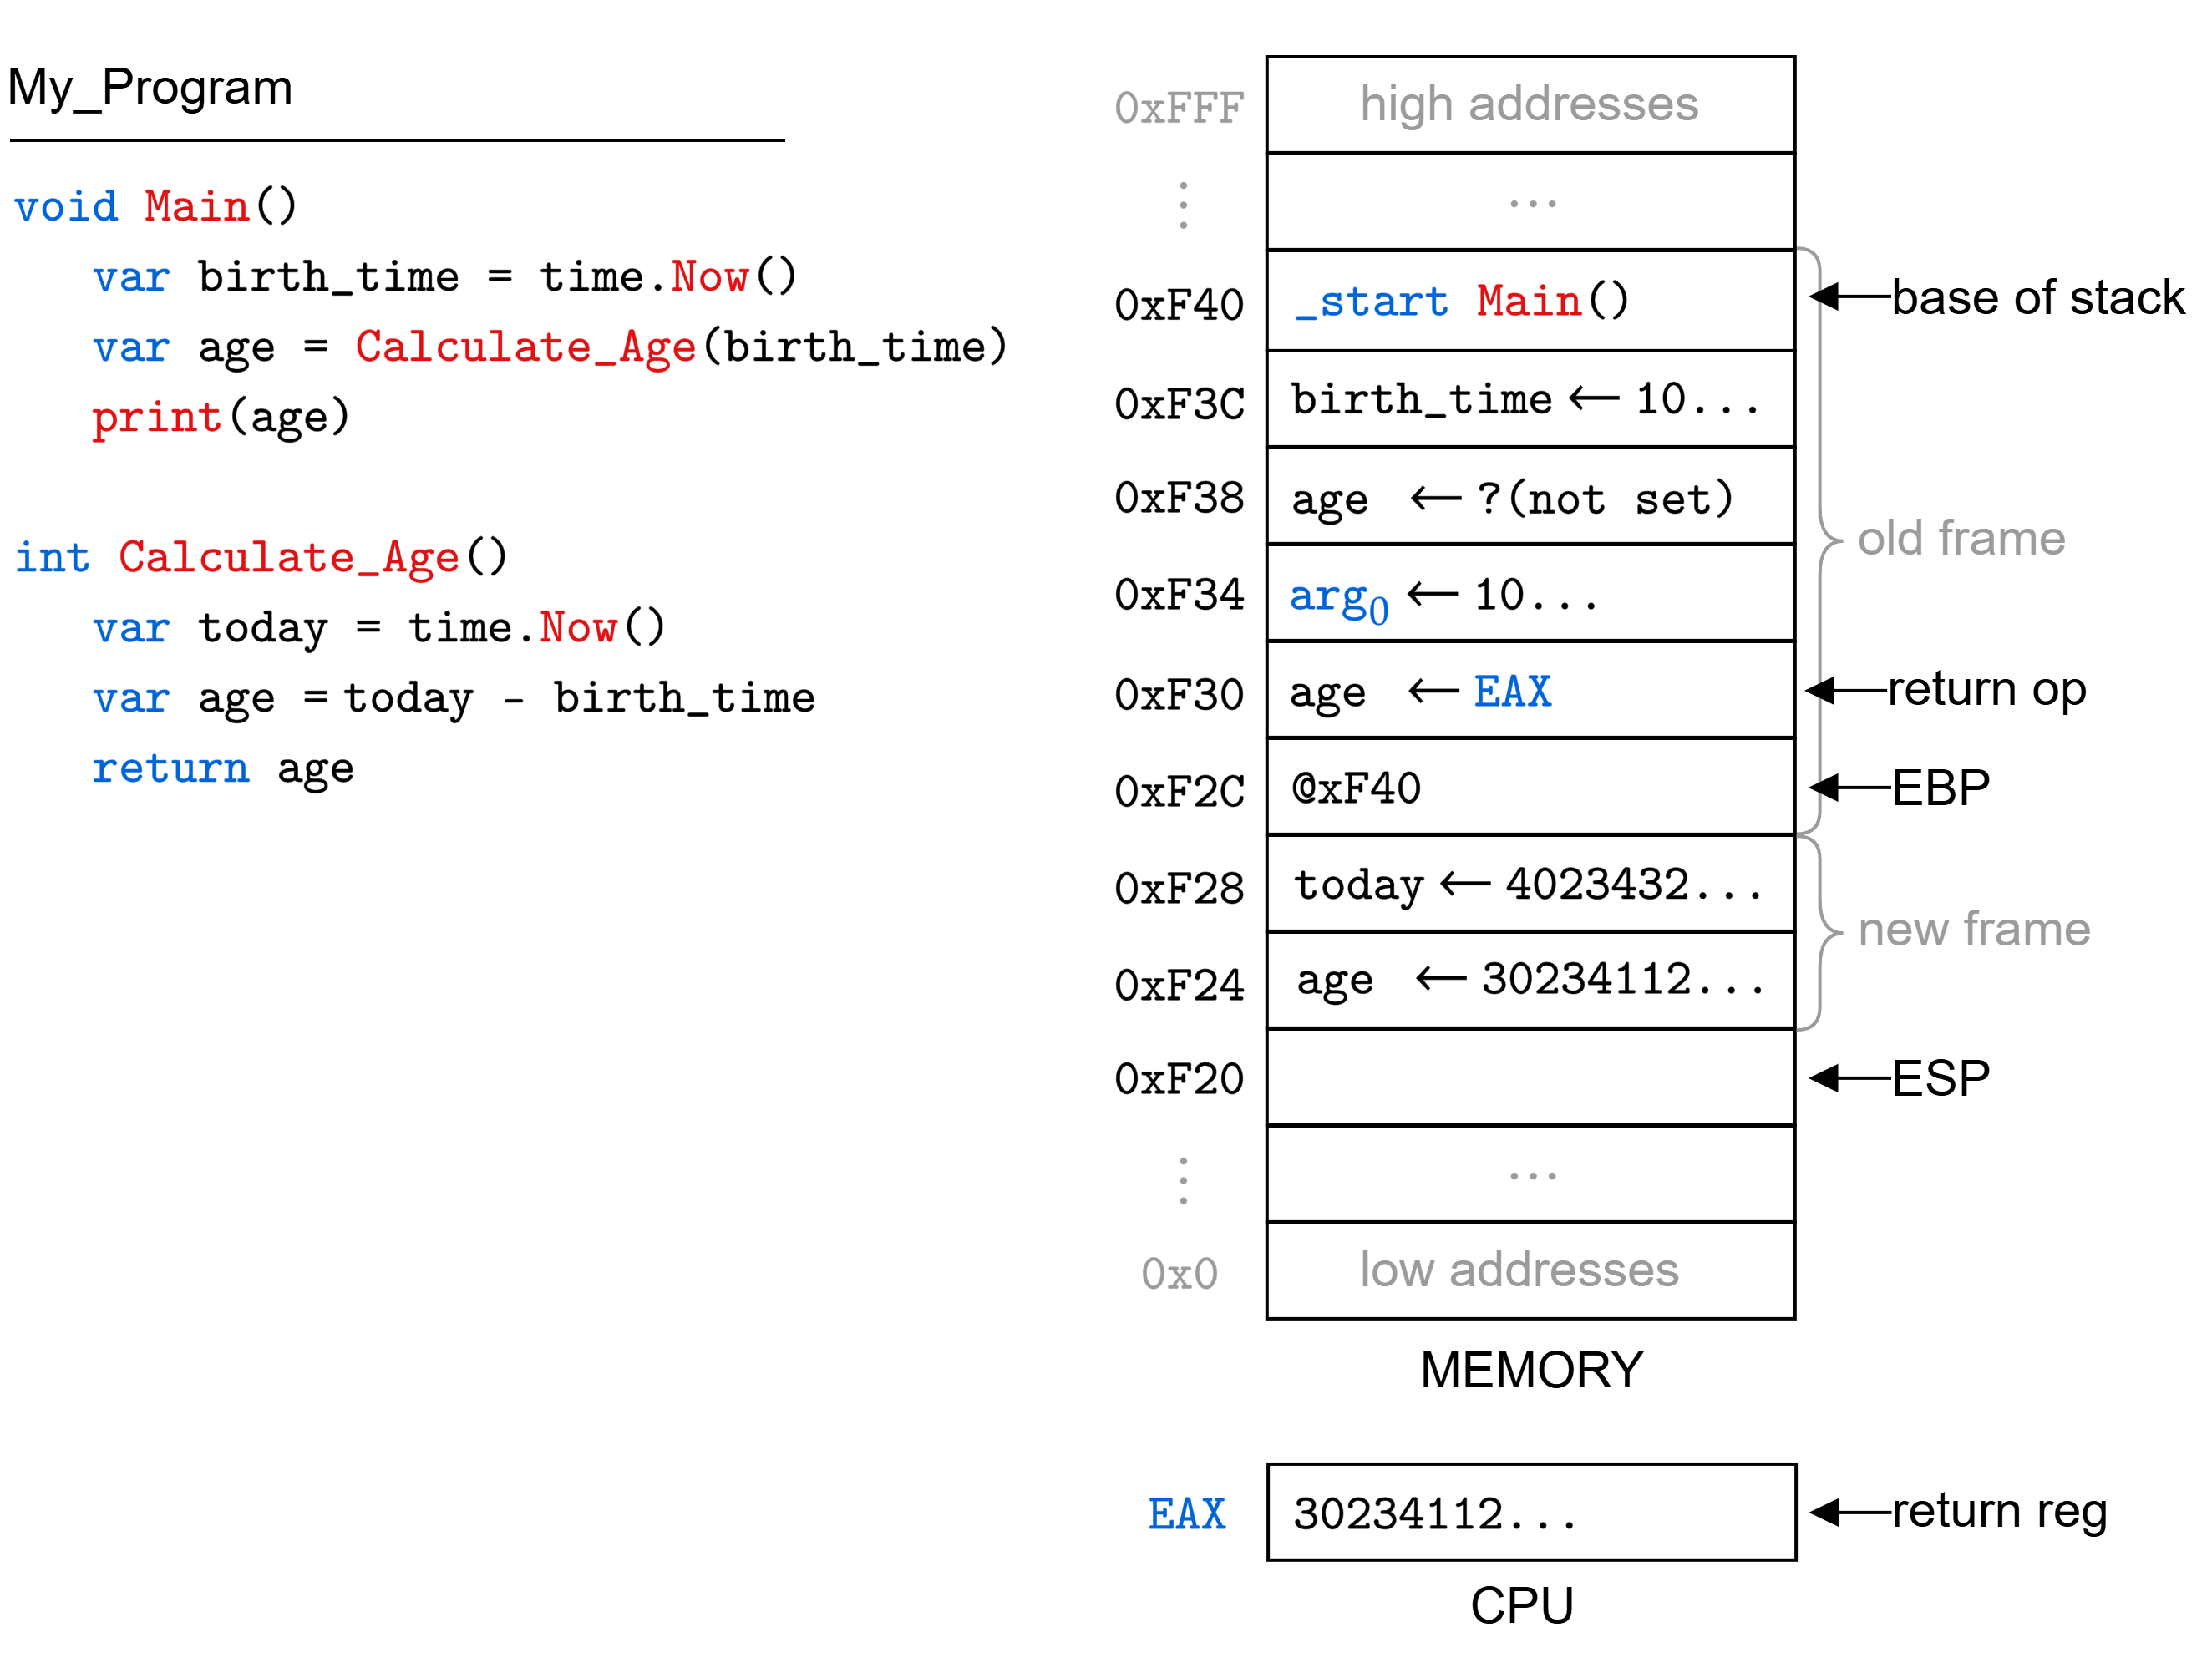
\includegraphics[width=\textwidth]{./Sections/stacks_heaps/call_stack_after.png}
    \caption{Revisiting Figure (\ref{fig:call_stack_precise}) at the moment the function \texttt{CalculateAge(birth\_time)} has supplied its return value to the EAX register, and is about to return.
    We see that before calling \texttt{CalculateAge(birth\_time)}: The old frame pushed it's arguments (\texttt{birth\_time}) onto the stack, then the return address (IP/Next Instruction) onto the stack,
    and finally the old EBP (Base Pointer) onto the stack. The `new frame' then sets the saved EBP address to the current EBP, concluding the old frame into the `new frame'. Moreover, since the offset
    looks for local variables below \texttt{0xF40}, the above `birth\_time' and `age' are \textbf{out of scope} for the `new frame', vice-versa. \textbf{Note:} This is 
    still a high-level abstraction of what actually happens sequentially with opcodes; Nonetheless, this is the fundamental idea of how a stack works. }
    \label{fig:call_stack_after}
\end{figure}

\noindent 
This concludes our discussion on stack structures; We continue with the heap structure next.

\newpage 

\noindent
\section{Heap Data Structures}
\label{sec:heap}

\noindent
So far we have simply said global data is declared in the \textbf{data segment} of memory. There is a second segment 
of memory that builds ontop of this called the \textbf{heap}:
\begin{Def}[Heap -- Dynamic vs. Static Memory]

    When a program runs there is a \textbf{static} (fixed) region reserved for the program's data segment (local/global variables). 
    During execution, more objects may be created, needing additional memory; A new region of memory is reserved \textbf{dynamically},
    building upwards from the top of the data segment, \underline{called the \textbf{heap}}.\\
    
    \noindent
    Language protocols either \textbf{manually} (e.g., Assembly, C) or \textbf{automatically} (e.g., Python, Java) manage this memory:
    \begin{itemize}
        \item \textbf{Manual Memory Management:} The programmer must explicitly allocate and deallocate memory using functions like `malloc' and `free' in C.
        \item \textbf{Automatic Memory Management:} The language runtime automatically allocates and deallocates memory, often using a \textbf{garbage collector} to reclaim unused memory (no variables pointing to it).
\end{itemize}

\noindent
Unlike the stack, this allows values to be accessed from anywhere in the program, regardless of the function call or scope.
\end{Def}

\noindent
We discuss hash tables more in-depth in the following section, for now we provide a high-level idea:
\begin{Def}[Hash Table]

    \label{def:hash_table}

    A \textbf{hash table} uses a \textbf{hash function}, taking a \textbf{key} (e.g., number or string) and producing a fixed-sized \textbf{hash} value (index),
    creating a table of mappings (key$\to$hash). At such indices lies data associated with the key, enabling fast data retrievals.

    A \textbf{universal hash function} is a hash function that uniformly distributes hashes across the hash table.

    \noindent
    \rule{\textwidth}{0.4pt}
    
    \noindent
    \textbf{Note:} The input in many context (typically cryptographic), may be called `data' or `message'; The output: hash, checksum, fingerprint, or digest.
\end{Def}
\begin{Def}[Arrays in Memory]

    Arrays list elements sequentially in memory. A reference to 
    an array is a pointer to the first element. To terminate reading an array, we must either know the size of said 
    array or have some \textbf{sentinel value} (e.g., `null' or `0') to indicate the end of the array.
\end{Def}
\newpage
\noindent
Consider the following examples:

\begin{figure}[ht!]
    \centering
    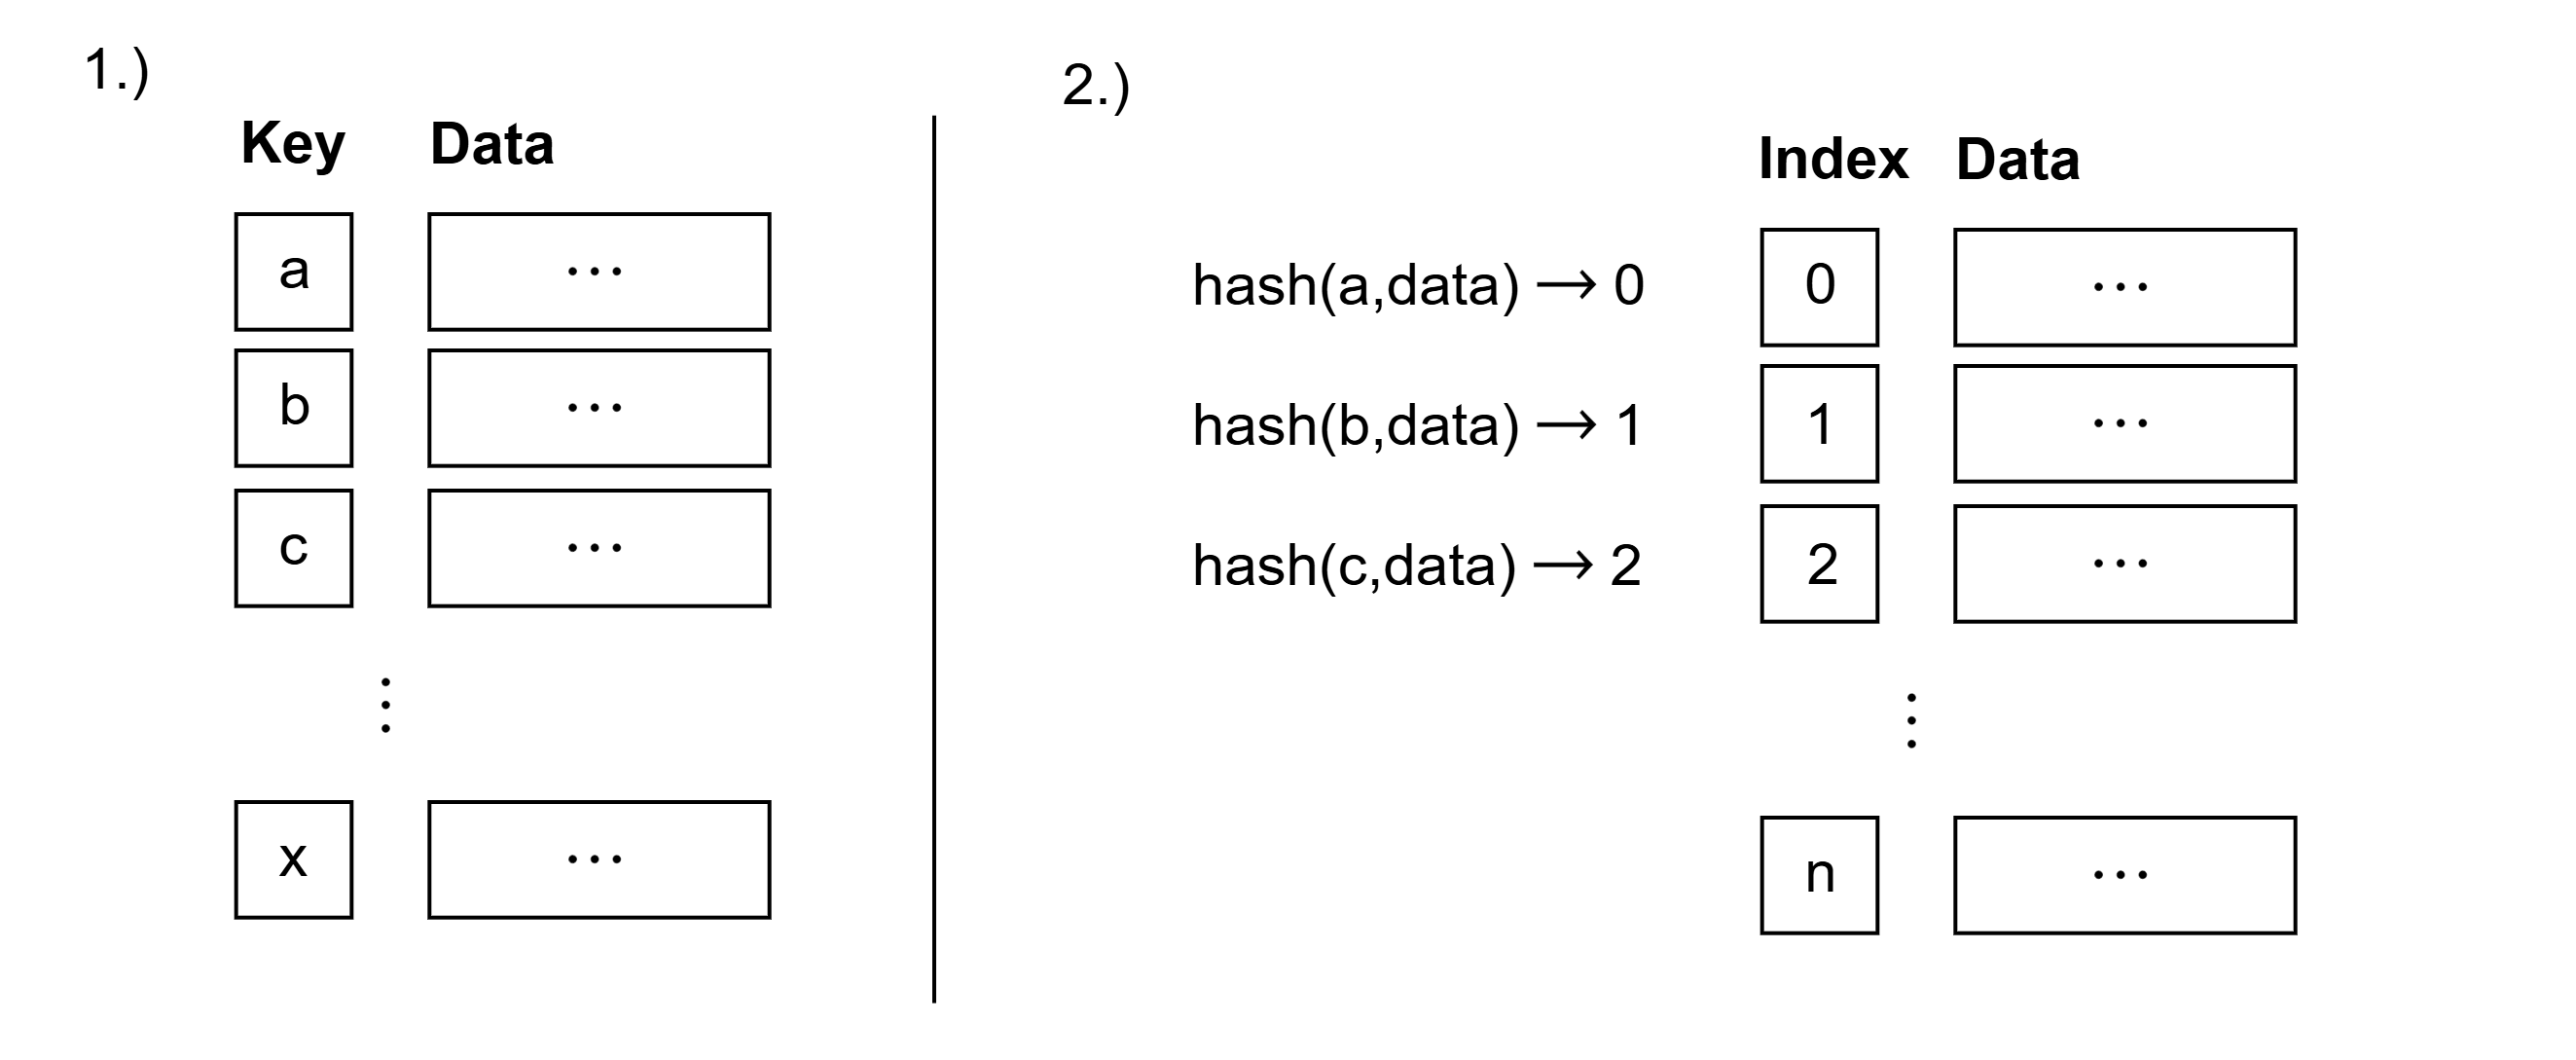
\includegraphics[width=\textwidth]{./Sections/stacks_heaps/hash_table.png}
    \caption{On the left (1) demonstrates a typical diagram one might find when learning about hash tables. Here $a$ through $x$ are the keys, which house some type of 
    data. On the right (2) shows a slightly more detailed version, which emphasizes that keys $a$--$x$ are hashed to indices $0$--$n$ in the hash table. The data could be any other 
    value (e.g., number, string, or object). Moreover, hash tables under the hood are arrays, with each index pointing to whatever data is associated with the key.}
    \label{fig:call_stack_after}
\end{figure}

\begin{figure}[ht!]
    \centering
    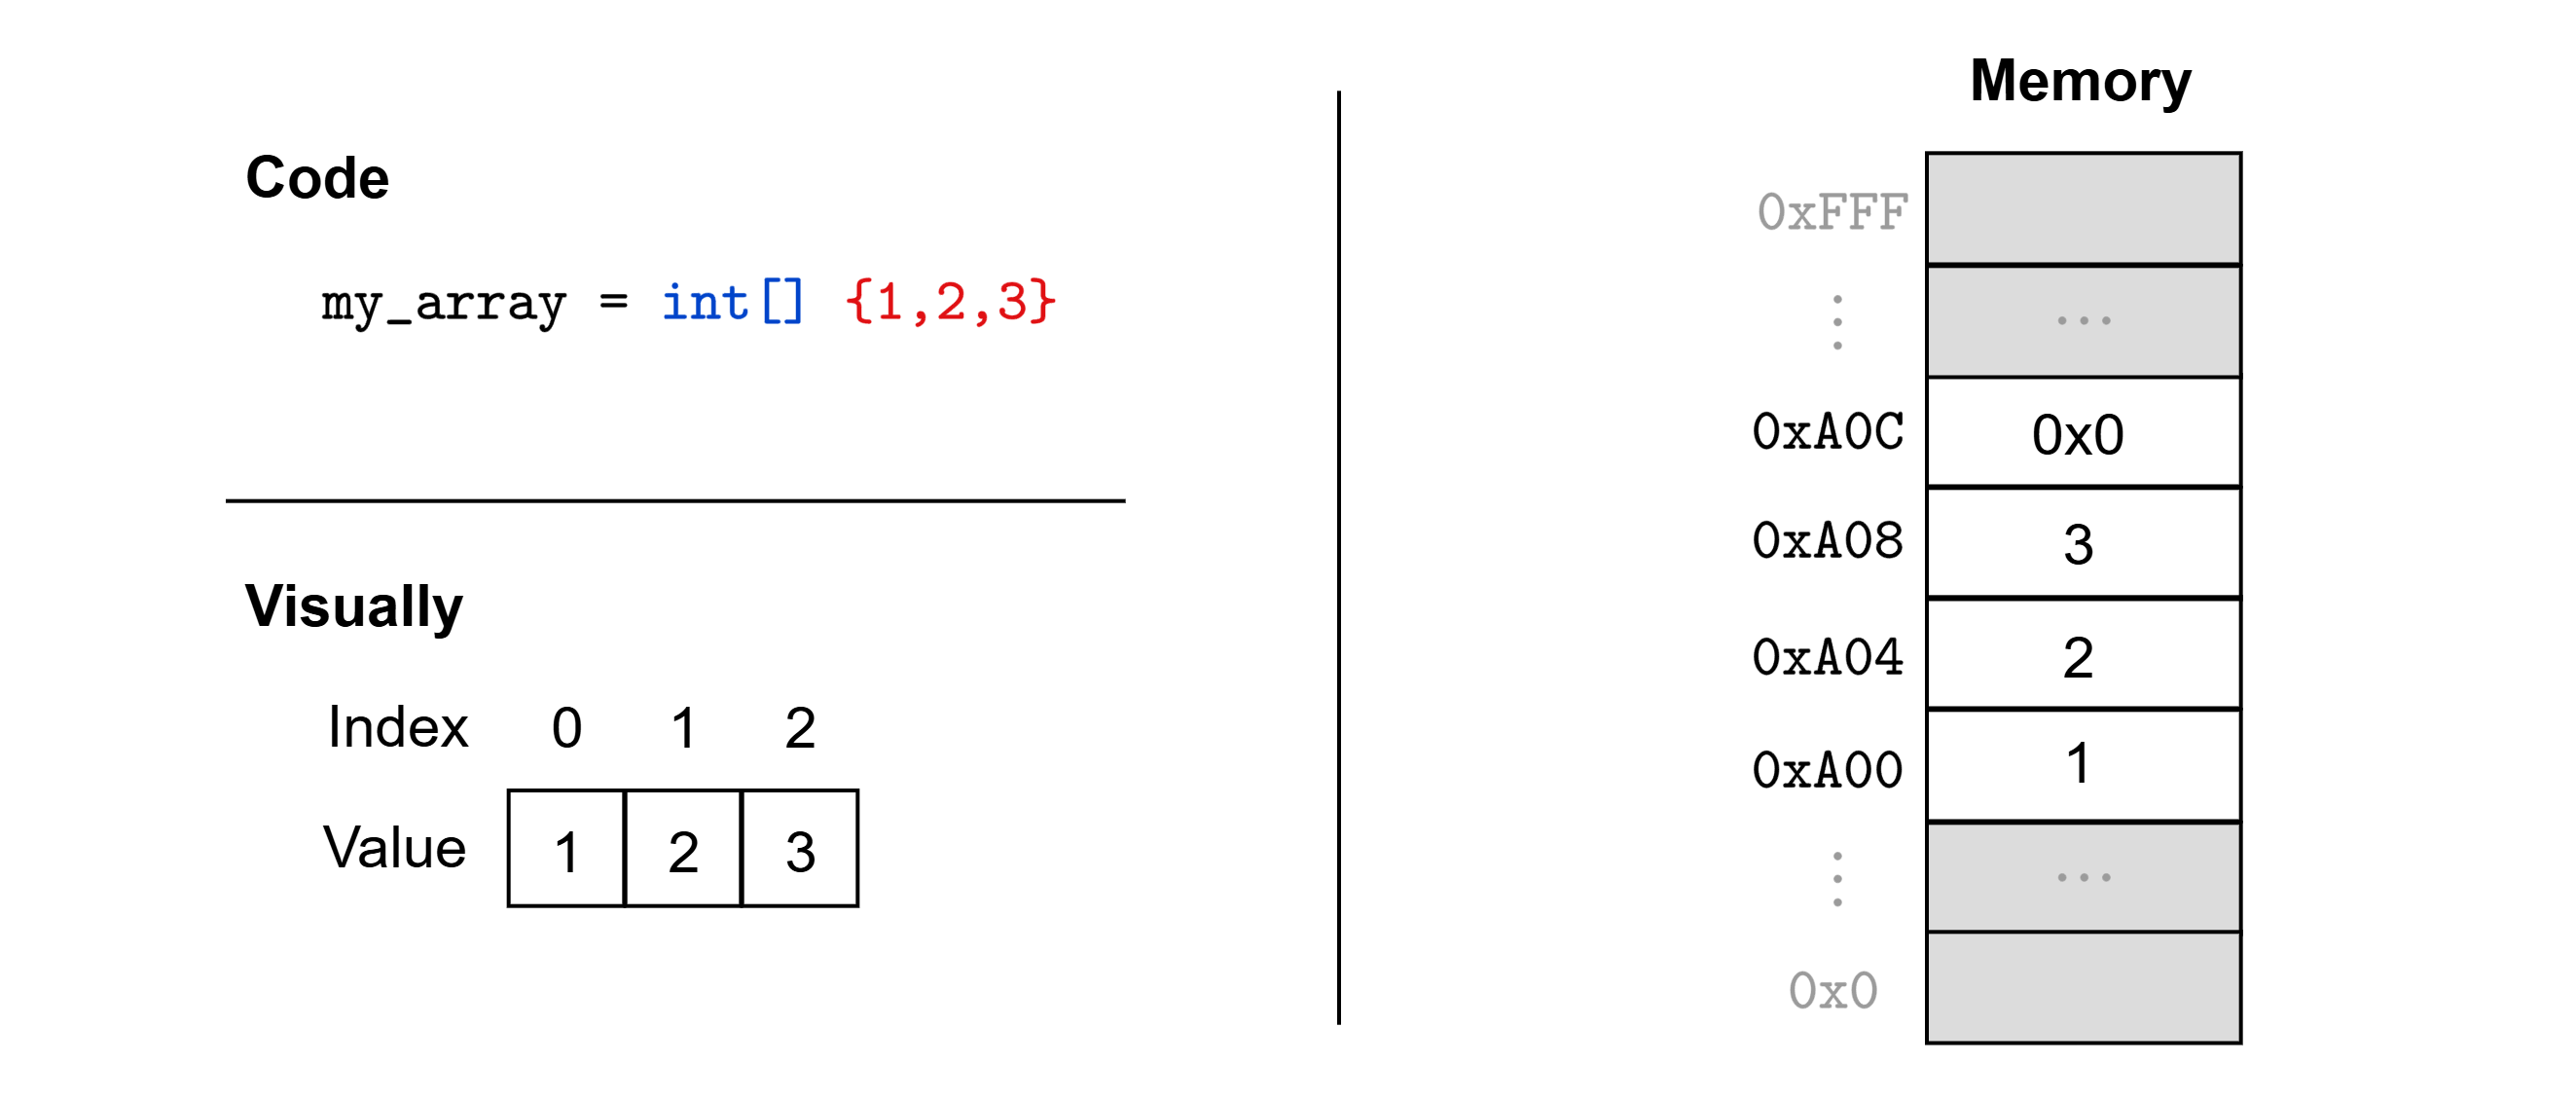
\includegraphics[width=\textwidth]{./Sections/stacks_heaps/arrays.png}
    \caption{Here there are three sections breaking down how arrays look: In code, typical diagram depictions (Visually), and in memory. The 
    code depiction illustrates a toy language creating an array of numbers ($[1,2,3]$). The visual depiction shows how indices relate to values. The 
    memory depiction shows how the array is laid out in contiguous memory locations, where \texttt{0x0} is the sentinel value (a bit-pattern of all zeros). 
    In code, \texttt{my\_array} holds the address \texttt{0xA00}.}
    \label{fig:array_memory}
\end{figure}

\newpage

\noindent
Objects behave very similarly to arrays, but with a few key differences:
\begin{Def}[Objects in Memory]

    An \textbf{Object} (or \textbf{struct}), is a collection of key-value pairs, 
    where each key is called a \textbf{field} or \textbf{attribute} and each value can be any data type (e.g., number, string, or address).

    Attributes are stored in array like fashion, where each element is a fixed-offset from the head (start) of the object.
    The object itself is a pointer to the first element. Accessing attributes works differently in compiled (e.g., C) vs. interpreted (e.g., Python) languages:
    \begin{itemize}
        \item \textbf{Compiled Languages:} There is no lookup, as the compiler has \emph{hardcoded} the offsets of each attribute interaction (e.g., `object.attribute' is translated to a direct memory access).
        \item \textbf{Interpreted Languages:} The interpreter looks up a hash table lookup for the attribute name.
    \end{itemize}

    \noindent
    Depending on the use case, objects may be stored in the heap or stack:
    \begin{itemize}
        \item \textbf{Static Objects:} An objects whose size is known at compile time can be allocated on the stack. I.e., no changes 
        to the object are made after creation (e.g., Math and Time objects, which purely exist to compute).
        \item \textbf{Dynamic Objects:} Often just called \textbf{objects}, are allocated on the heap, allowing for dynamic resizing and modification (e.g.,
        a student object with attributes like `name', `age', and `grades' that can change over time).
    \end{itemize}

    \noindent
    Languages like Java push this even further by allowing both static (shared) and dynamic (personal) fields within a class.
\end{Def}

\noindent 
We define the following for completeness sake:
\begin{Def}[Classes \& Interfaces]

    Object-oriented programming is a paradigm where objects are the main building blocks of the program.
    A \textbf{class} is a blueprint for defining how an object will behave once \textbf{instantiated} (created). In this paradigm,
    functions are called \textbf{methods}, as they are defined and used within the class (i.e., globally does not exist in independence).\\

    \noindent
    Some languages (e.g., Java, C++) support \textbf{interfaces} (or protocols), which specify a set of methods that implementing classes must provide. Although the terminology varies 
    (abstract classes, traits, protocols, etc.), they all ultimately describe capabilities an object must fulfill.
\end{Def}

\newpage 

\noindent
Strings are not what they seem:
\begin{Def}[Strings \& Characters in Memory]

    \noindent
    A \textbf{character} is represented by a numeric code unit:
    \begin{itemize}
      \item In C, a single \texttt{char} (1 byte) typically holds an ASCII code (0--127). Characters beyond U+FFFF use two \texttt{char} values, a \textbf{surrogate pair}.
      \item In Java, \texttt{char} is a 16-bit UTF-16 code unit (U+0000..U+FFFF). ASCII values (0--127) map directly to the same Unicode code points. We can take advantage of the encoding:
      
    \begin{lstlisting}[language=Java]
    char c = 'A';
    System.out.println((int)c);  // prints 65, since 'A' is U+0041
    \end{lstlisting}
      
      \noindent
      This allows us to do things like checking for 
      valid characters:
    \begin{lstlisting}[language=Java]
    if ((c >= 'a' && c <= 'z') || (c >= 'A' && c <= 'Z')) {
        // c is in 'a'..'z' or 'A'..'Z'
    }
    \end{lstlisting}

    \noindent
    We can also perform arithmetic on \texttt{char}:
    \begin{lstlisting}[language=Java]
    char c = 'A';               // U+0041 (65)
    char next = (char)(c + 1);  // 'B' (66)
    \end{lstlisting}
    \end{itemize}
    
    \noindent
    \rule{\textwidth}{0.4pt}\\ 

    \noindent
    \underline{Typically, a \textbf{string} is stored as a contiguous array of \textbf{characters}.} In low-level languages (e.g.\ C),
    that array ends with a null terminator (\verb|\0|) and literal strings reside in the data segment. 
    In higher-level languages (e.g.\ Java, Python), strings are full objects with methods. For e.g.,\\

    \noindent
    \textbf{C:}  
    \begin{itemize}
      \item String literals (e.g.\ \texttt{"Hello"}) are placed in the (often read-only) data segment.
      \item Runtime-constructed strings (via \texttt{malloc}, \texttt{strcpy}, etc.) live on the heap.
    \end{itemize}

    \noindent
    \textbf{Java:}  
    \begin{itemize}
      \item Compile-time literals are \textbf{interned} (stored as a single shared copy) into the \textbf{String Constant Pool} section (specially reserved on the heap).  
      \item Any other \texttt{String} (e.g.\ via \texttt{new String(...)}, concatenation, or user input) also resides on the heap but outside the pool.  
      \item Because Java strings are immutable, interning lets multiple references share the same character data.
    \end{itemize}

    
\end{Def}

\newpage

\noindent
With slight alterations to our code in Figure (\ref{fig:call_stack_after}), we illustrate heaps and arrays:

\begin{figure}[!ht]
    \centering
    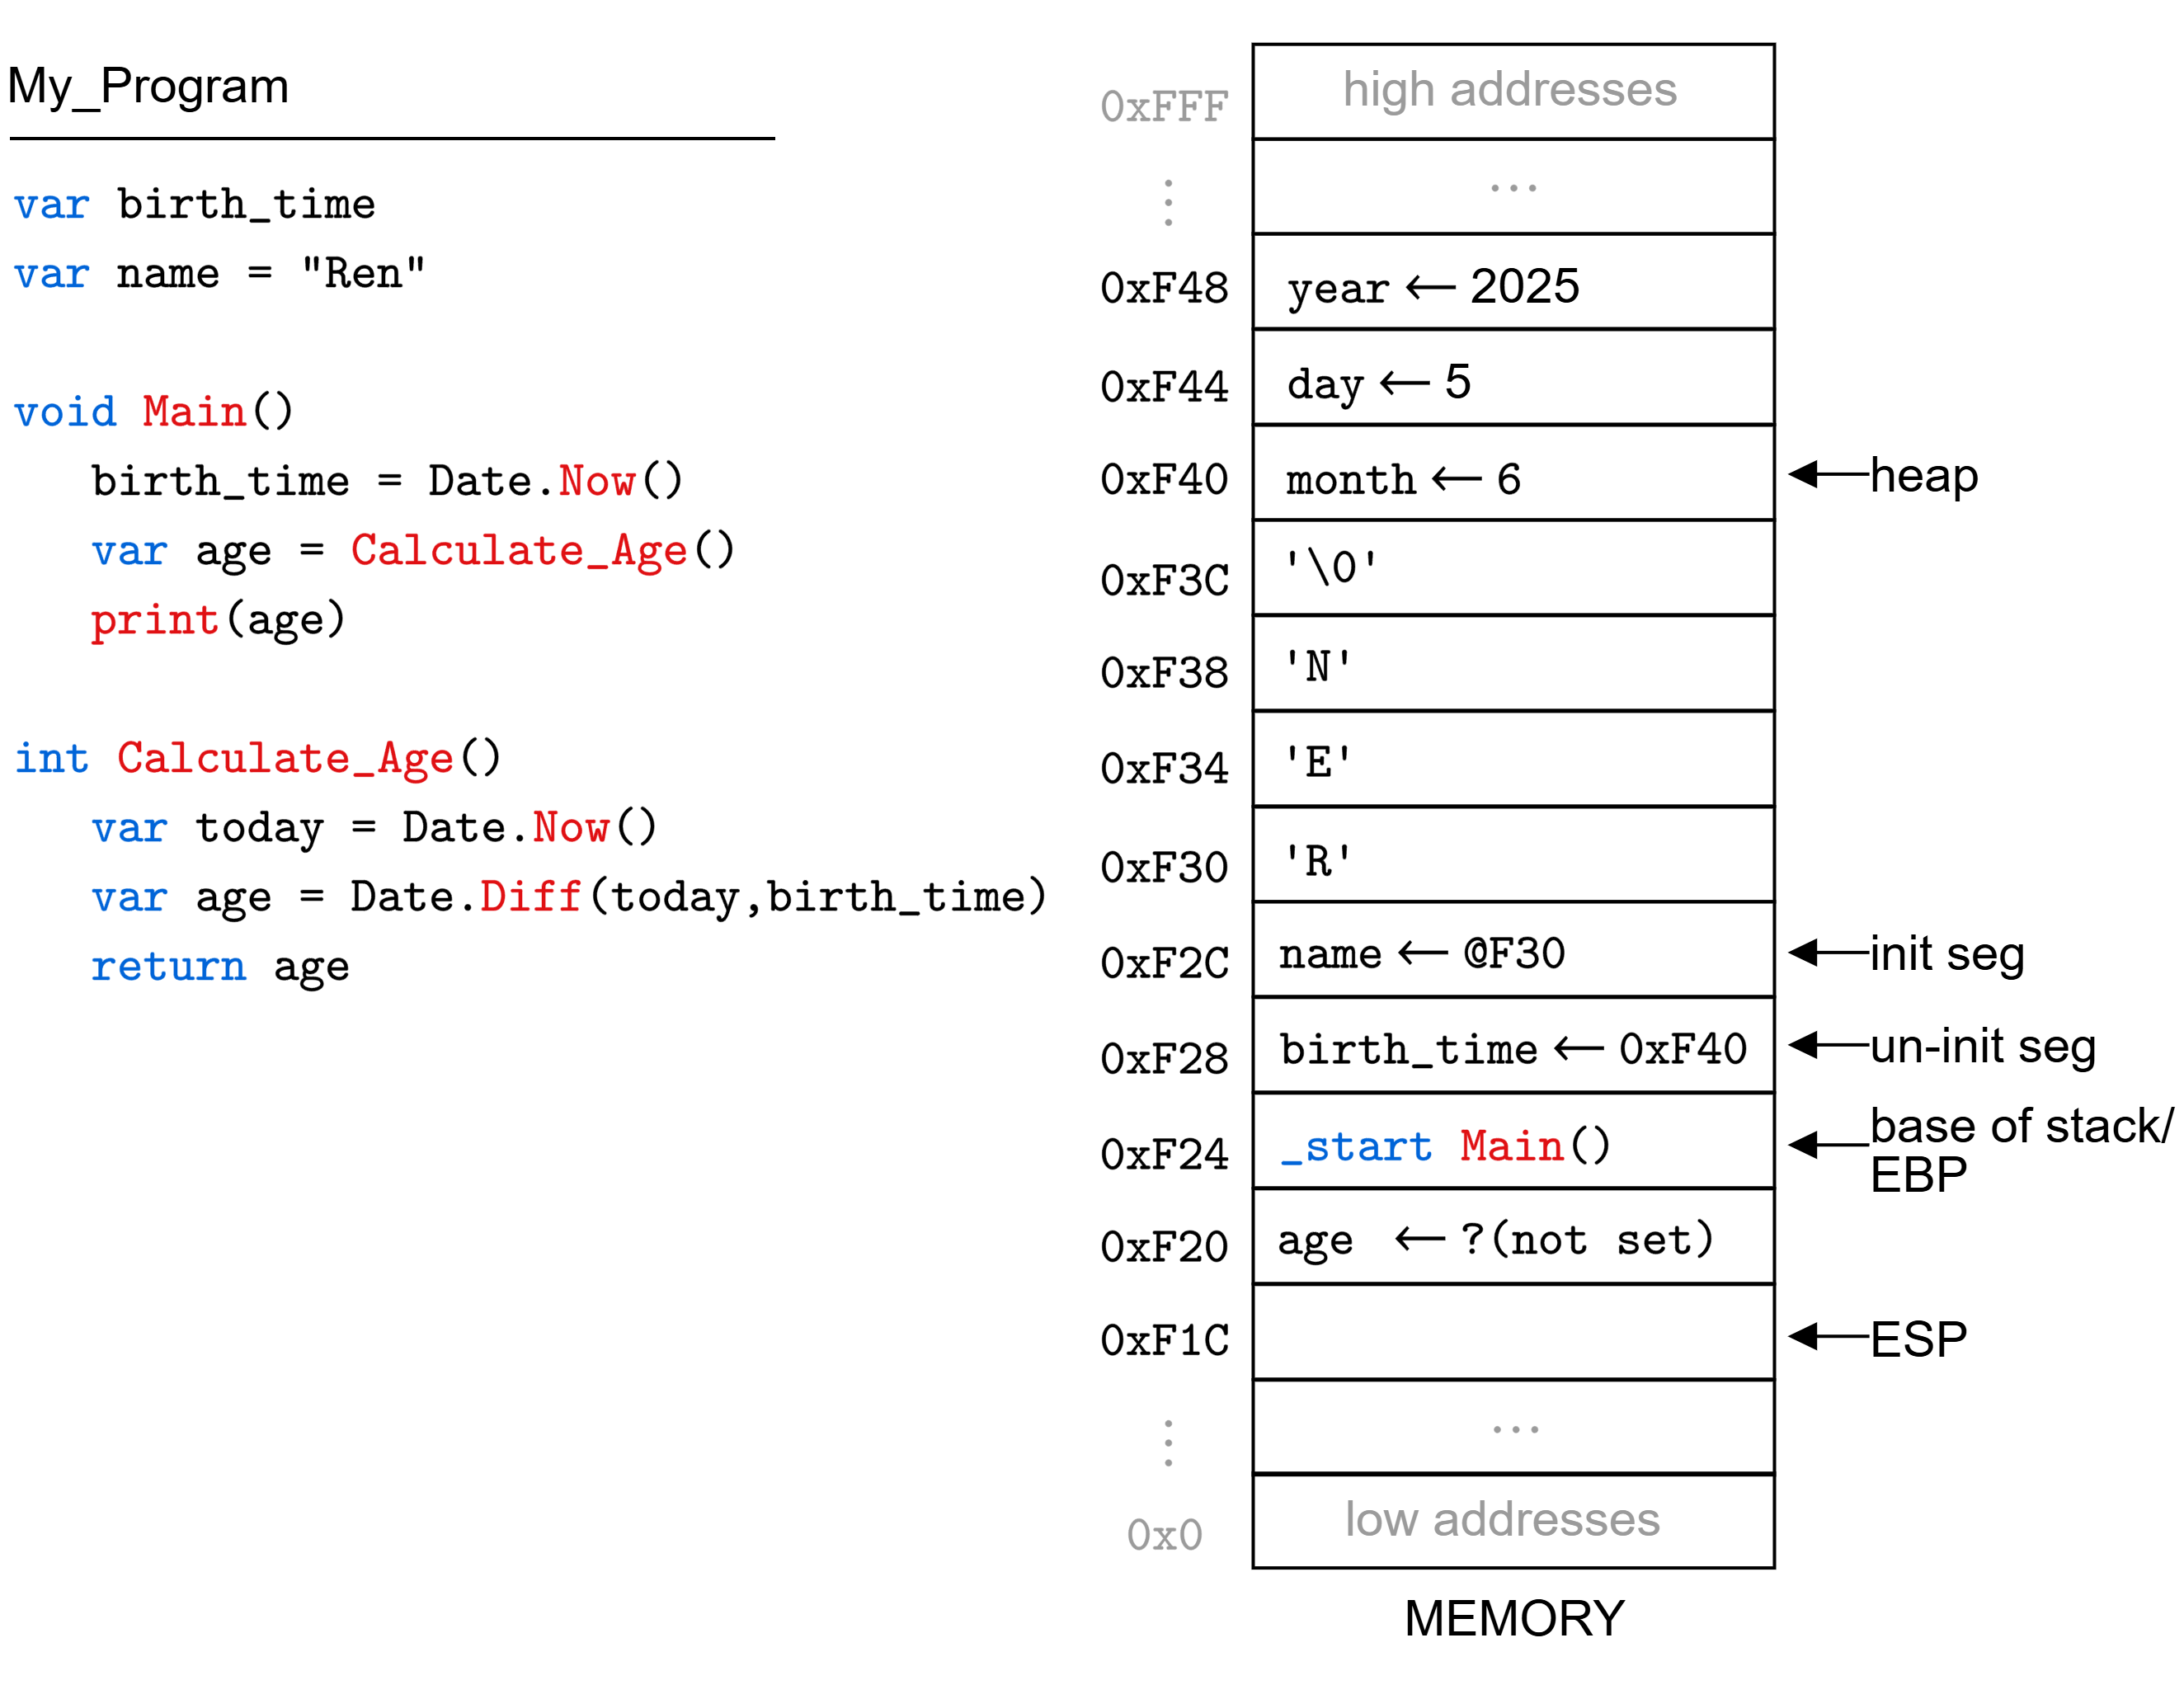
\includegraphics[width=\textwidth]{./Sections/stacks_heaps/heap_array.png}
    \caption{Here \texttt{birth\_time} and \texttt{name} are global variables. Following the C convention, \texttt{birth\_time} is placed in the 
    uninitialized data segment, while \texttt{name} is placed in the initialized data segment. Since \texttt{name} is a string, it holds a 
    reference to the first character in the string, which is stored contiguously in the initialized data segment ending with a null terminator (`\texttt{\textbackslash 0}').
    During execution, \texttt{Date.Now()} a method call from a \texttt{Date} object is called; This method returns a new object, which is placed on the heap with 
    its attributes (\texttt{month}, \texttt{day}, \texttt{year}) stored contiguously in memory. \textbf{Note:} Methods such as \texttt{Date.Diff()} are code (not data), 
    which do not live in the heap or stack.}
    \label{fig:heap_array}
\end{figure}

\begin{Def}[Factory Method]

    A \textbf{factory method} is a function that creates and returns an object, often initializing it with default values or parameters.
    In Figure (\ref{fig:heap_array}), the method \texttt{Date.Now()} is a factory method that creates a new \texttt{Date} object with the current date and time.
\end{Def}

\noindent
The below illustration summarizes the heap and stack in memory:
\begin{figure}[!ht]

    \hspace{-6em} 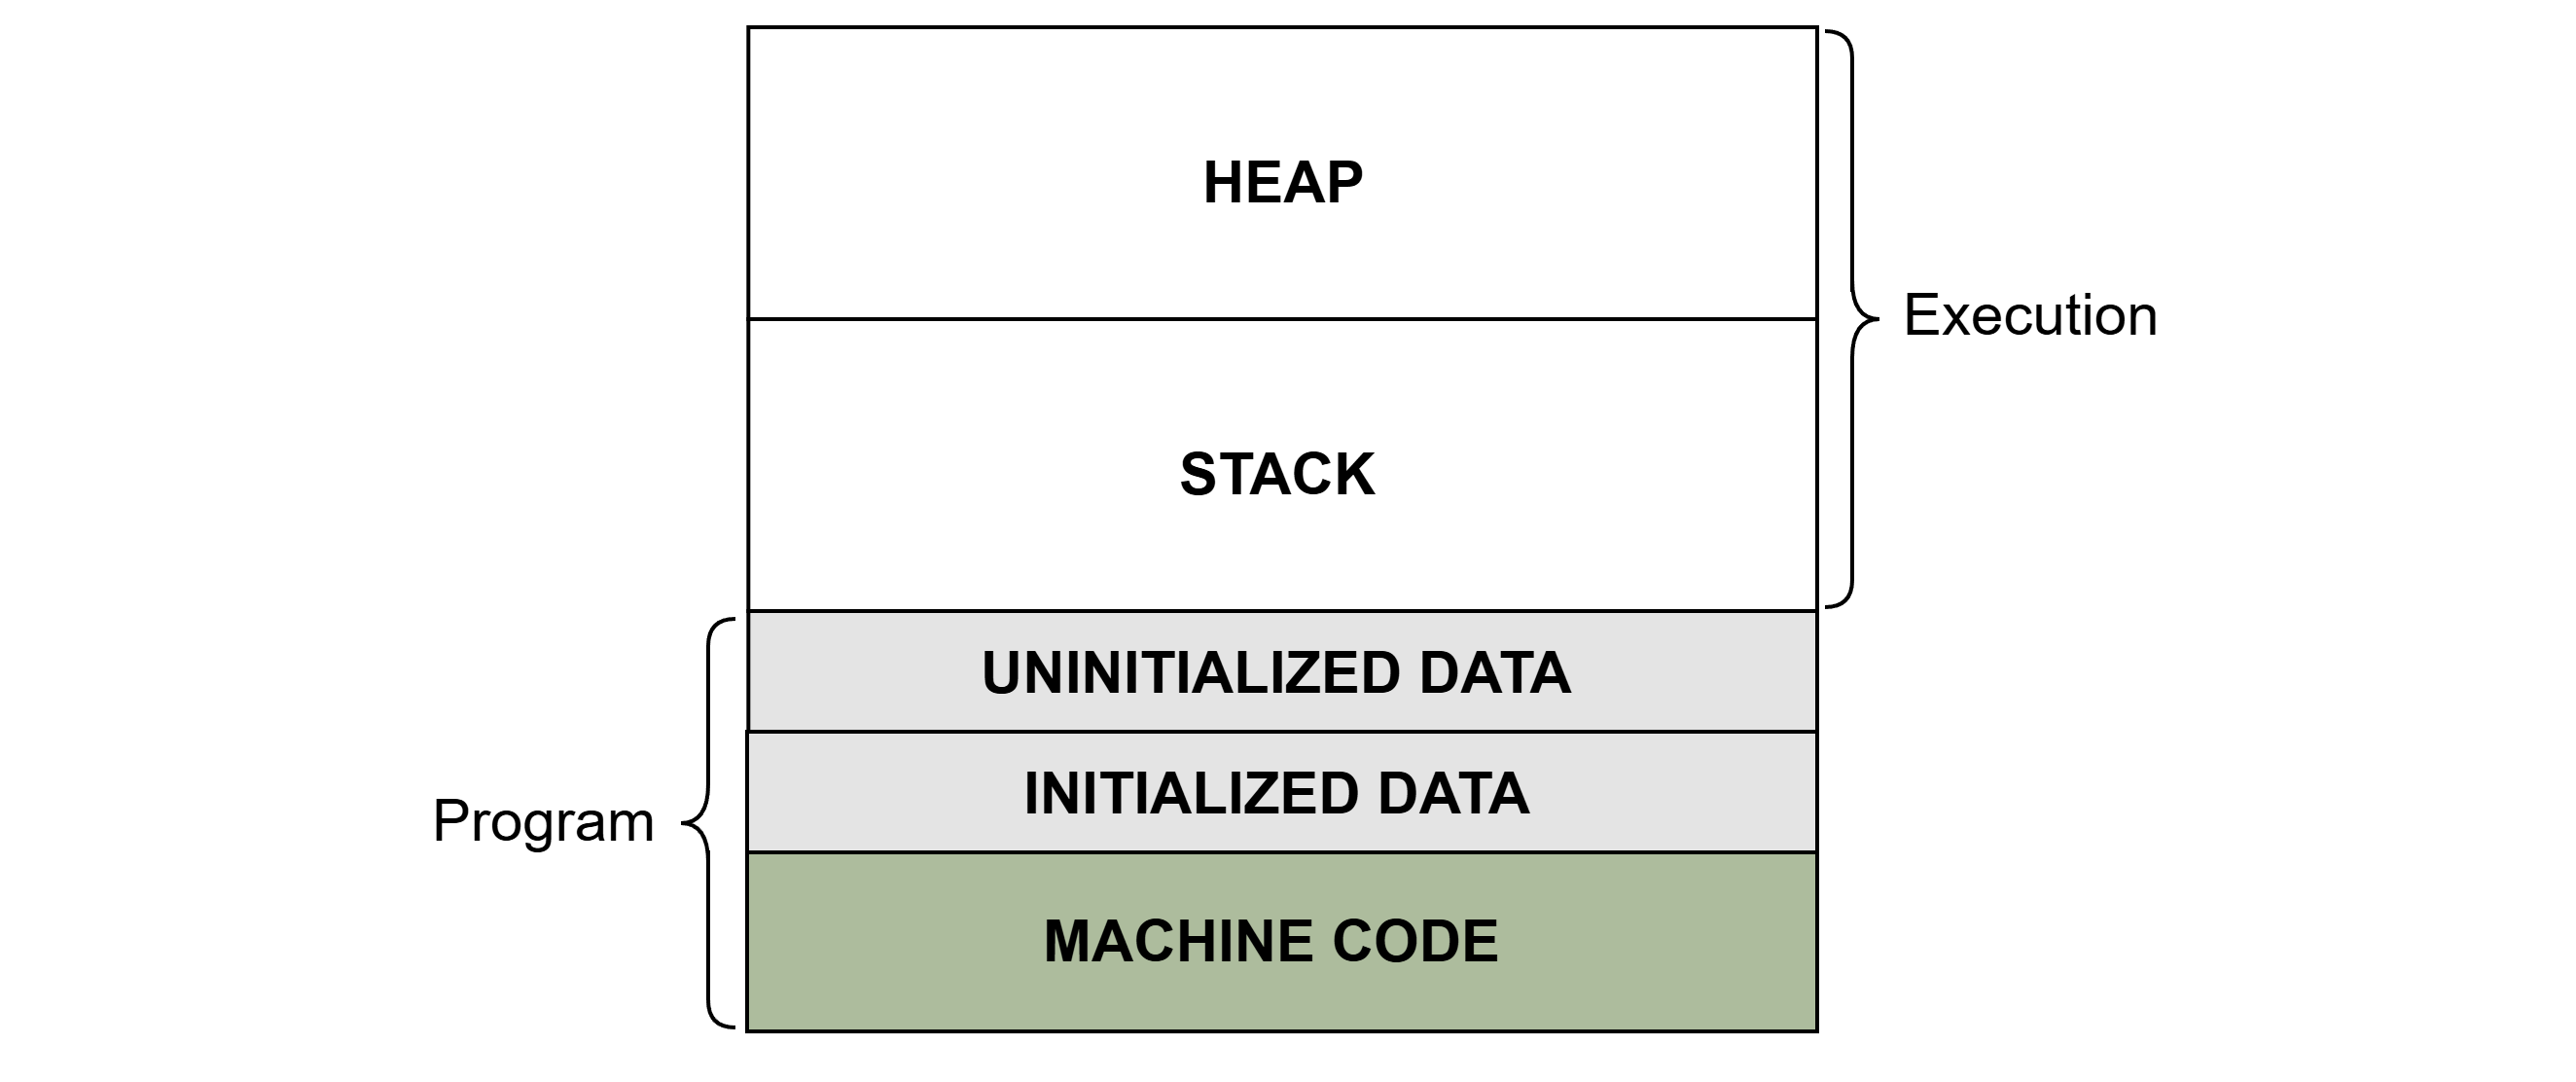
\includegraphics[width=1.3\textwidth]{./Sections/stacks_heaps/stack_heap_memory.png}
    \caption{The above figure demonstrates the relationship from bottom-to-top the order at which data is 
    loaded into memory. First the program compiles to machine code and loaded by the OS into memory.
    From there, provisions to the data segment (static memory: uninitialized and initialized) are made. Depending 
    on the OS, some objects may have already been loaded into the heap, which are referenced by initialized data segment variables.
    Then as functions are called, the stack grows downwards within its allotted memory space. During execution of each stack frame,
    new objects may be placed on the heap, referenced by variables in the stack or data segment. Then depending on the language,
    a garbage collector periodically checks for objects with no references (i.e., no variables pointing to them) and deallocates them;
    Alternatively, the program explicitly deallocates memory using functions like `free' in C.}
    \label{fig:stack_heap_memory}
\end{figure}